\section{Related Work}\label{sec:related}
% Fig. 1 defined here so that it floats to the top of page 3, after Related Work starts (user 2026-11-18).
\begin{figure*}[t]
\centering
% Source: figures/src/fig_c2d2_standalone.tex + latex/figures/fig_c2d2.tex (TikZ), built by build.sh (user 2026-11-13: training and network in two figures).
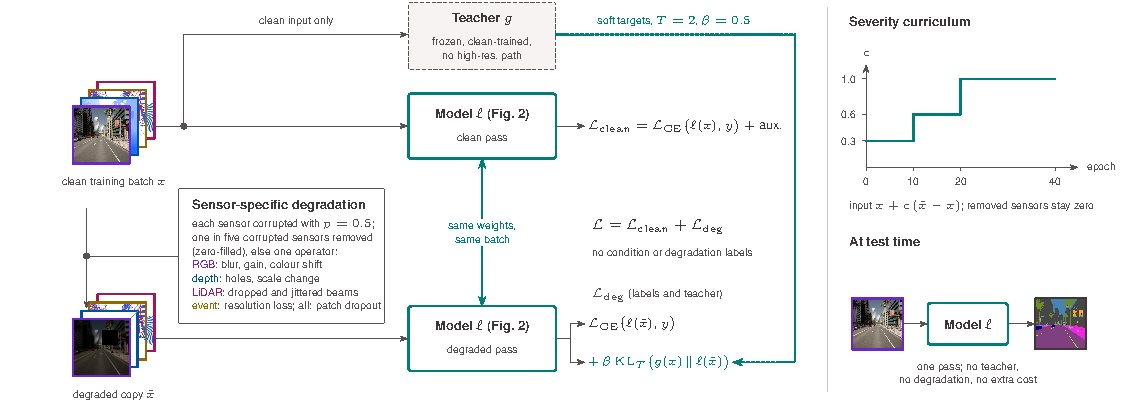
\includegraphics[width=\textwidth]{figures/fig_c2d2.pdf}
\caption{Training with C2D2. Every batch is used twice by the same model (Fig.~\ref{fig:arch}): a clean pass on the original samples, and a degraded pass on a copy in which each sensor is corrupted with probability $p$, either removed (zero-filled) or degraded by a sensor-specific operator. The degraded pass is supervised by the labels $y$ and by the soft targets of a frozen teacher that sees the clean input (Section~\ref{sec:m_c2d2}); a curriculum raises the degradation severity during the first epochs. Only the model is used at test time, in one pass. Teal outlines mark trained components and dashed boxes frozen weights.}
\label{fig:overview}
\end{figure*}
% Comparison table and audit for this section: repo .claude_logs/research/novelty-and-related-work.md and
% research/2026-10-20-structural-novelty-audit.md. Bibliography checked 2026-10-28 (notes/reference_check.md).

\subsection{Multimodal Fusion for Segmentation}
Early RGB-X segmentation fused one auxiliary sensor into an RGB stream, for example by cross-modal feature rectification~\cite{cmx2023} or by exchanging tokens between modality-specific transformers~\cite{tokenfusion2022}. CMNeXt~\cite{cmnext2023} generalized this to an arbitrary number of sensors with a hub that aggregates the auxiliary sensors before injecting them into RGB, and introduced DELIVER. Later work improved efficiency and accuracy with adapter-based early fusion~\cite{stitchfusion2024} and pixel-level token exchange~\cite{geminifusion2024}. CAFuser~\cite{cafuser2025} conditions the fusion on the scene condition inferred from the camera image, and DGFusion~\cite{dgfusion2026} uses depth, with depth supervision, to guide the fusion; both report leading results on DELIVER and MUSES. These methods are designed and evaluated with all sensors present. We re-train two of them with synthetic degradation and modality dropout (without distillation) and compare them with our model under one protocol (Section~\ref{sec:exp}).

\subsection{Robustness to Missing and Degraded Sensors}
A second line of work trains models that tolerate missing sensors. MAGIC~\cite{magic2024,magicpp2024} treats all modalities equally and, during training, ranks modality features by their similarity to an aggregated feature. AnySeg~\cite{anyseg2024} names the problem unimodal bias, the over-reliance on a dominant, faster-to-learn modality, and reduces it by distilling a multimodal teacher into a student trained with random modality dropout; functional-entropy regularization~\cite{zheng2025entropy} targets the same bias. RMMSS~\cite{rmmss2025} combines prototype distillation with feature selection. A recent benchmark~\cite{mmssbench2025} standardized entire-missing, random-missing, and noisy-modality evaluations, which we adopt, and attributed robustness differences to fusion design. FuseAdapt~\cite{fuseadapt2026} adapts a frozen DINOv2 backbone with modality-private low-rank adapters that exchange residual activations, and adds a training objective in which an exponential-moving-average teacher with all sensors supervises the prediction of the representation of a masked sensor. Methods in this line usually skip a missing input, whereas the benchmark protocol replaces it with zeros; we keep the two families apart when comparing numbers.

\subsection{Distillation from Clean to Degraded Inputs}
Supervising a model on degraded inputs with the predictions of a teacher that sees the clean input is an established recipe. Su and Maji~\cite{su2017cqd} train a recognition model on synthetically degraded images (low resolution, edges, distortion) with a label loss plus a distillation loss towards a model trained on the clean images, the same form as our degraded-pass loss; adversarially robust distillation~\cite{goldblum2020ard} applies it with adversarial inputs, and later work distills high-resolution teachers into low-resolution face recognizers~\cite{shin2022askd} and clean-image detectors into students trained on corrupted, downscaled images~\cite{lee2026cdfkd}. For dense prediction, md4all~\cite{gasperini2023md4all} supervises depth estimation on translated night and rain images with a teacher run on the original daytime images, and RobustSAM~\cite{chen2024robustsam} keeps the features of a degraded image consistent with those of its clean counterpart. In multi-sensor segmentation, the student input is usually perturbed by removing sensors: AnySeg~\cite{anyseg2024} and RMMSS~\cite{rmmss2025} distill a full-sensor teacher into a student with randomly dropped modalities, M3L~\cite{maheshwari2023m3l} and MMANet~\cite{wei2023mmanet} distill towards models with complete inputs in semi-supervised and incomplete-modality settings, and CRM~\cite{shin2024crm} enforces consistency between two randomly masked views of RGB-thermal inputs. Passing clean and perturbed copies of the same batch through one model is also used: SDSTrack~\cite{hou2024sdstrack} distills the clean path into a masked path of a frozen tracker with adapters, UniMRSeg~\cite{zhao2025unimrseg} aligns predictions on complete and incomplete inputs, and Compass~\cite{liu2026compass} distills between an original and a modality-dropped stream. In all of these multi-sensor methods, the student is perturbed by removing or masking sensors. Training with sensor-specific simulated faults has so far been explored mainly for camera--LiDAR fusion: PFS~\cite{dong2026pfs} samples camera and LiDAR corruptions independently to train a post-fusion module on top of a frozen detector without any teacher, and VG-SAF~\cite{tao2026vgsaf} pairs clean and fault-injected inputs within each single-sensor expert, pulling the noisy prediction toward the stop-gradient clean prediction of the same network. To our knowledge, no prior work combines the two lines, that is, distills a frozen, separately trained clean-input teacher into a degraded pass in which each of up to four sensors is independently either removed or corrupted by a sensor-specific operator. C2D2 does this; what we study is its effect on a fusion model built on a frozen foundation backbone, measured under a public missing- and noisy-sensor protocol.

\subsection{Adapting Frozen Foundation Models}
Vision foundation models are increasingly used as frozen encoders for dense prediction. The Segment Anything Model~\cite{sam2023} has been adapted to multimodal inputs with adapters that inject auxiliary-sensor features into the RGB stream~\cite{mmsamadapter2025} or with mixtures of LoRA experts~\cite{mlesam}, and MemorySAM~\cite{memorysam2025} reuses the memory mechanism of SAM~2~\cite{sam2_2024} to fuse modalities. DINOv3~\cite{dinov3_2025} provides dense features and a segmentation adapter derived from ViT-Adapter~\cite{vitadapter2023}, which we reuse for our high-resolution path. Our backbone, LoRA adaptation~\cite{lora2022}, and query head~\cite{mask2former2022} build on these works; we treat them as the platform for our study, not as contributions.
